\section{Method}


\subsection{Design of the Framework}

In our framework, we employ multiple LLM-based agents working collaboratively to detect errors in KGs. Using the structural information of the graph, we construct four bidirectional subgraph agents for both the head and tail entities. These agents analyze the contextual information of triples from different perspectives, and a final decision on the correctness of the triples is made through a voting mechanism. The detailed explanation of this process is provided below:

\textbf{Bidirectional Subgraph Agents: }
%
%
%
In our MAKGED framework, we design four bidirectional subgraph agents to evaluate triples in the knowledge graph. Each of these agents is responsible for analyzing triples from a specific directional perspective, including the \textit{Head\_Forward\_Agent} and \textit{Head\_Backward\_Agent} for the head entity, and the \textit{Tail\_Forward\_Agent} and \textit{Tail\_Backward\_Agent} for the tail entity, as illustrated in Figure~\ref{framework}.


First, we construct bidirectional subgraphs for both the head and tail entities of each triple. For the head entity, the \textit{Head\_Forward\_Agent} extracts the \textit{Out\_Neighbor subgraph}, where the edges represent outgoing relations from the head entity; concurrently, the \textit{Head\_Backward\_Agent} extracts the \textit{In\_Neighbor subgraph}, where the edges represent incoming relations directed toward the head entity. Similarly, for the tail entity, the \textit{Tail\_Forward\_Agent }and \textit{Tail\_Backward-
\_Agent} generate forward and backward subgraphs, representing the tail entity as either a head node or a tail node in related subgraphs.

\begin{figure*}
  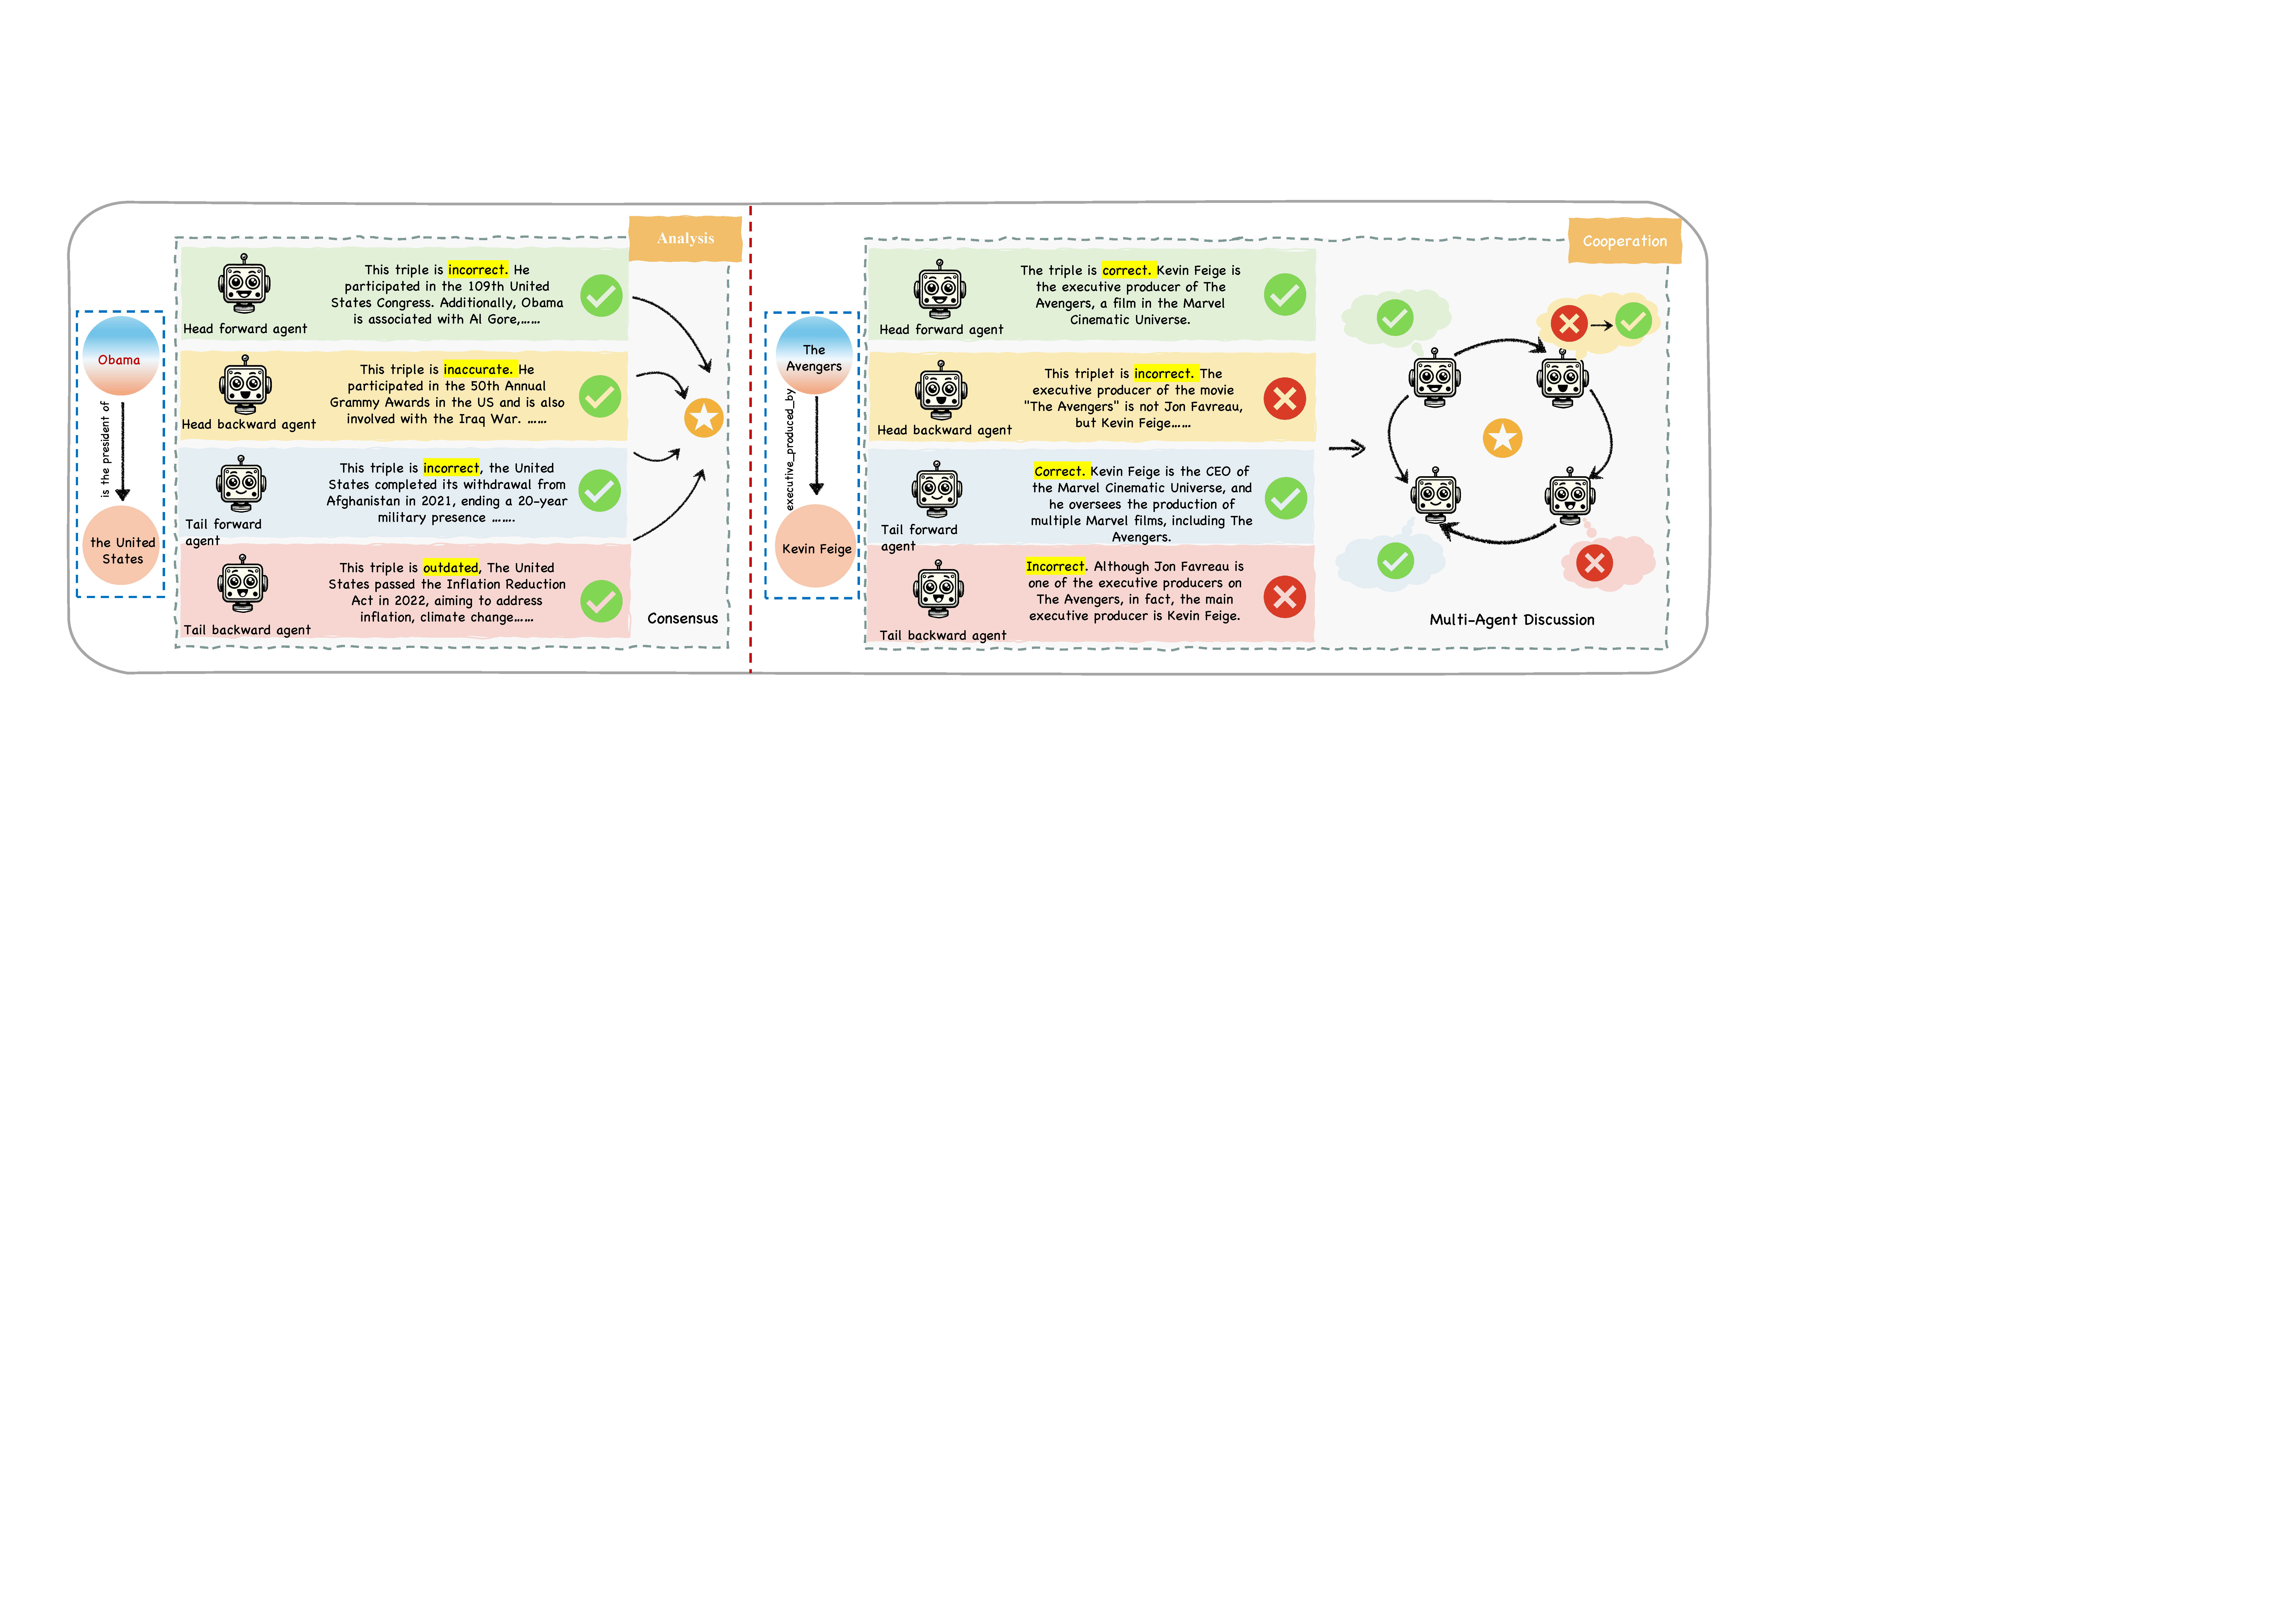
\includegraphics[width=1\textwidth]{fig2.pdf}
  \caption{This figure illustrates the collaborative decision-making process using multiple agents. In the "analysis" phase, the four agents independently evaluate the triple. If no consensus is reached, they proceed to the "cooperation" phase for discussion. The final decision is made either by majority rule after three rounds of discussion, or by a summarizer in case of a  \textit{2-vs-2} tie.}
  \label{agent}
\end{figure*}


Once the subgraphs are constructed, we process them using a Graph Convolutional Network to generate the corresponding subgraph embedding vectors. Let the subgraph embeddings be denoted as \( \mathbf{z}_{G} \). These subgraph embeddings are then concatenated with the embedding vectors generated by Llama2, denoted as \( \mathbf{e}_{text} \), which provides textual information for assessing the correctness of the triples. Llama2 embeddings provide the textual representation of the triples, while the structural information from the subgraph embeddings adds complementary context. By concatenating both semantic and structural information, we create a richer, more expressive unified embedding representation:

\begin{align}
    \mathbf{e}_{concat} = [\mathbf{z}_{G} ; \mathbf{e}_{text}]
\end{align}

where \(\mathbf{z}_{G}\) denotes the graph-based embeddings generated by the GCN module. \(\mathbf{e}_{text}\) represents the semantic embeddings derived from Llama2.
Next, these concatenated embeddings are used as input to further fine-tune the Llama2 model. During fine-tuning, the model learns not only how to combine textual and structural embeddings to improve its accuracy but also how to optimize its decision-making based on the distinct features of the subgraphs in each direction. The input sequence to the model is defined as:
% 
\begin{align}
    S_{it} = I_{it} \oplus \mathbf{e}_{concat} \oplus A_{it},
\end{align}
% 
where \( I_{it} \) is the instruction prompt, \( \mathbf{e}_{concat} \) is the concatenated embedding from both the GCN and Llama2, and \( A_{it} \) is the predicted answer during training. 
% We compute the loss by comparing the model's output with the ground truth labels. 
The training objective is to minimize the following loss function:

\begin{align}
    \mathcal{L}_{it} = - \frac{1}{|S_{it}|} \sum_{i=1}^{|S_{it}|} \log P_{\mathcal{M}}(s_i \mid s_{<i}, \mathbf{e}_{concat}), 
\end{align}
% 
where \( |S_{it}| \) represents the length of the input sequence \( S_{it} \), and \( s_i \) is the token at position \( i \) in the input sequence. \( P_{\mathcal{M}}(s_i \mid s_{<i}, \mathbf{e}_{concat}) \) is the probability distribution predicted by the model for token \( s_i \), conditioned on all previous tokens and the concatenated embedding.
% 
During the training process, we simultaneously train the Llama2 to evaluate the correctness of triples in scenarios where reasoning is provided. In this part, subgraph information is incorporated into the input, allowing the model to fine-tune its ability to discuss the correctness of triples based on reasoning.

As a result, we train four specialized agents, each tailored to specific directional tasks for either the head or tail entities (forward or backward). This method allows us to comprehensively evaluate the correctness of triples from multiple directions, significantly enhancing the performance and accuracy.



\textbf{Agent Decision: }
%
The agents trained in the previous process are used for the KG error detection task on the test set. This process is divided into two phases: the analysis phase and the cooperation phase. In the analysis phase, the four agents (\textit{Head\_Forward\_Agent} and \textit{Head\_Backward\_Agent} for the head entity, and \textit{Tail\_Forward\_Agent} and \textit{Tail\_Backward\_Agent} for the tail entity) evaluate the correctness of a target triple independently, making full use of the corresponding subgraph information they learned during training and minimizing mutual interference.

After collecting the results, a consistency check is performed. If all agents agree on the correctness of the triple (i.e., consensus), it is classified as correct or incorrect. If there is disagreement, the process moves to the cooperation phase.

In the cooperation phase, the four agents engage in a collective discussion, exchanging their viewpoints and background knowledge to resolve disagreements regarding the triple. This discussion process iterates for up to three rounds, stopping early if consensus is reached within these rounds. After each round of discussion, the agents update their judgments. At the end of the discussion, a ``majority rule'' strategy is employed to determine the final decision. If a \textit{2-vs-2} tie still occurs after the three rounds, 
the final decision is made by a summarizer agent, which receives the full context of the three discussion rounds as a structured prompt. This prompt includes key arguments, evidence, and conclusions from all agents, enabling the summarizer to make an informed judgment that reflects the collective reasoning of the agents.
On average, in our experience, agents reached a consensus within 1.8 rounds of discussion. In about 12\% of cases, a \textit{2-vs-2} tie occurred, which was resolved by the summarizer agent.
The entire agent discussion process is illustrated in Figure \ref{agent}.

